\section{Same Sign Di-leptons}
\label{sec:samesign}

This section summarizes the results of the SUSY parameter space scan
in the same sign di-lepton channel. The measurement strategy is  
described in detail in a previous CMS note~\cite{ssnote}. The technique
utilizes two data-driven methods to estimate background characterized
by the presence of two isolated high $P_T$ same sign leptons,
$\met$, and significant hadronic activity.  For the purpose 
of this note we restrict ourselves to the $ee$, $e\mu$, and $\mu\mu$
final states, {\em i.e.}, we do not consider $\tau$'s, except in the
case that the $\tau$ decays leptonically. 

As we will show in Section~\ref{sec:ssyields}, for a reasonable event
selection the main background is from \ttbar decays. The data-driven background 
prediction is based on a combination of estimating ``fake leptons''~\cite{fakenote} (FakeRate) 
and electrons reconstructed with the wrong sign~\cite{ssnote} (Charge FlipRate). The probability
for muons to be reconstructed with the wrong sign at the relevant momenta is negligible.

\subsection{Event Yields}
\label{sec:ssyields}

The expected SM event yields in 100~pb$^{-1}$ after applying the event selections
described in Section~\ref{sec:eventselection} to the datasets described in
Section~\ref{sec:datasamples} are detailed below

\vspace{6 mm}
\begin{table}[hbt]
\begin{center}
%\small\addtolength{\tabcolsep}{-5pt}
\renewcommand{\arraystretch}{1.2}
 {\footnotesize
\begin{tabular}{|l|c|c|c|c|c|c|c|c|}\hline
Same Sign leptons & Total SM & \ttbar & Single top & WZ & ZZ & WW & DY & Wjets \\ \hline

$ee$ & 0.07$\pm$0.04 & 0.06$\pm$0.04 & 0.00$\pm$0.00 & 0.01$\pm$0.01 & 0.00$\pm$0.00 & 0.00$\pm$0.00 & 0.00$\pm$0.00 & 0.00$\pm$0.00 \\
$\mu\mu$ & 0.09$\pm$0.05 & 0.09$\pm$0.05 & 0.00$\pm$0.00 & 0.00$\pm$0.00 & 0.00$\pm$0.00 & 0.00$\pm$0.00 & 0.00$\pm$0.00 & 0.00$\pm$0.00 \\
$e\mu$ & 0.22$\pm$0.08 & 0.21$\pm$0.08 & 0.00$\pm$0.00 & 0.01$\pm$0.01 & 0.00$\pm$0.00 & 0.00$\pm$0.00 & 0.00$\pm$0.00 & 0.00$\pm$0.00 \\ 
total & 0.38$\pm$0.10 & 0.36$\pm$0.10 & 0.00$\pm$0.00 & 0.02$\pm$0.01 & 0.00$\pm$0.00 & 0.00$\pm$0.00 & 0.00$\pm$0.00 & 0.00$\pm$0.00 \\ \hline
\end{tabular} }
\caption{Expected number of SM events passing the event selection in 100 pb$^{-1}$ of integrated 
luminosity. Uncertainties are from MC statistics.\label{tab:ssyields}}
\end{center}
\end{table}

The dominant SM contribution is from \ttbar decays. The total estimated background 
is obtained after the application of Fake and Charge Flip rates to the entire ensemble
of SM samples. The results of the application of the procedure is summarized in Table~\ref{tab:sm_preditcion}.

\begin{table}[hbt]
\begin{center}
\begin{tabular}{|l|c|}\hline
Sample & Event yield \\ \hline
Total SM (Observed) & 0.38 $\pm$ 0.10 \\
Total SM (Predicted) & 0.36 \\
\hline
\end{tabular}
\caption{ Observed and predicted number of SM events passing the event selection in 100 pb$^{-1}$ of integrated luminosity. The uncertainty is from Monte Carlo statistics.\label{tab:sm_preditcion}}
\end{center}
\end{table}


We then apply the same sign di-lepton event selection to the mSUGRA scan points. The resulting
event yield is shown in Figure~\ref{fig:ss_eventyield} for 100 pb$^{-1}$ of integrated luminosity.
LO cross sections has been used for the normalization. 

\vspace{3 mm}
\begin{figure}[htb]
\begin{center}
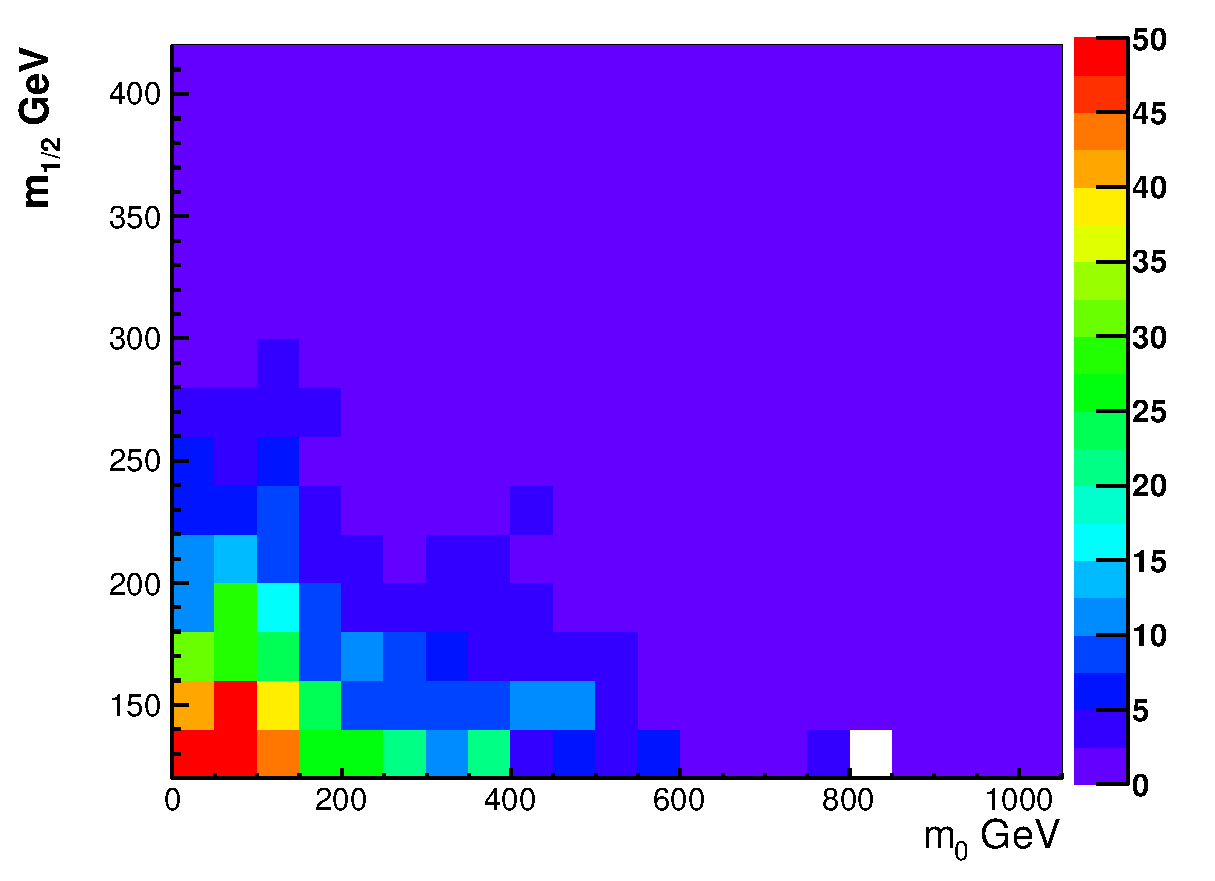
\includegraphics[width=0.7\linewidth]{figs/eventyieldss.eps}
\caption{Expected event yields in the mSUGRA $m_{0}-m_{1/2}$ plane with tan$\beta = 3$, A$_0 = 0$, $\mu > 0$
using 100 pb$^{-1}$ of integrated luminosity. The one white spot is a sample for which the MC statistics is low enough that not one generated event passed all cuts. Details on ``raw event yields'' are listed in the Appendix in Tables 6,7,8. \label{fig:ss_eventyield}}
\end{center}
\end{figure}


\subsection{Procedure for Determining $5\sigma$ Discovery Reach}
\label{sec:significance}

The $5\sigma$  discovery reach is estimated in the $m_{0}-m_{1/2}$
plane by  performing our analysis at each of the  mSUGRA scan points.
Expected event yields are based on the number of events passing
all cuts and scaled by the LO cross section for that point with 100 pb$^{-1}$ or 1 fb$^{-1}$ 
of simulated events respectively. We apply both of the above mentioned data-driven 
estimation procedures to determine the ``signal contamination'' at each of the benchmark points. 
The significance is quantified by the observed yield and the predicted background
using estimators: $Z_{Bi}$~\cite{cite:cousins}  and $Z_{N}$\cite{cite:conway}. The following
are used in order to compute the significance:
\begin{itemize}
\item The predicted background yield.
\item The relative systematic  uncertainty on the predicted background
yield (set to 50\%).
\item The  statistical uncertainty  on the predicted  background yield
($Z_N$ only, set to 0).
\item The observed yield.
\item The MC-based signal yield.

\end{itemize}
Figures~\ref{fig:ss_zn} and~\ref{fig:ss_zbi} show the discovery reach for various 
luminosity scenarios in one of the mSUGRA planes using $Z_{N}$ and $Z_{Bi}$ respectively.
Clearly, a large region of phase space can be accessed using higher luminosity. 
\vspace{3 mm}
\begin{figure}[htb]
\begin{center}
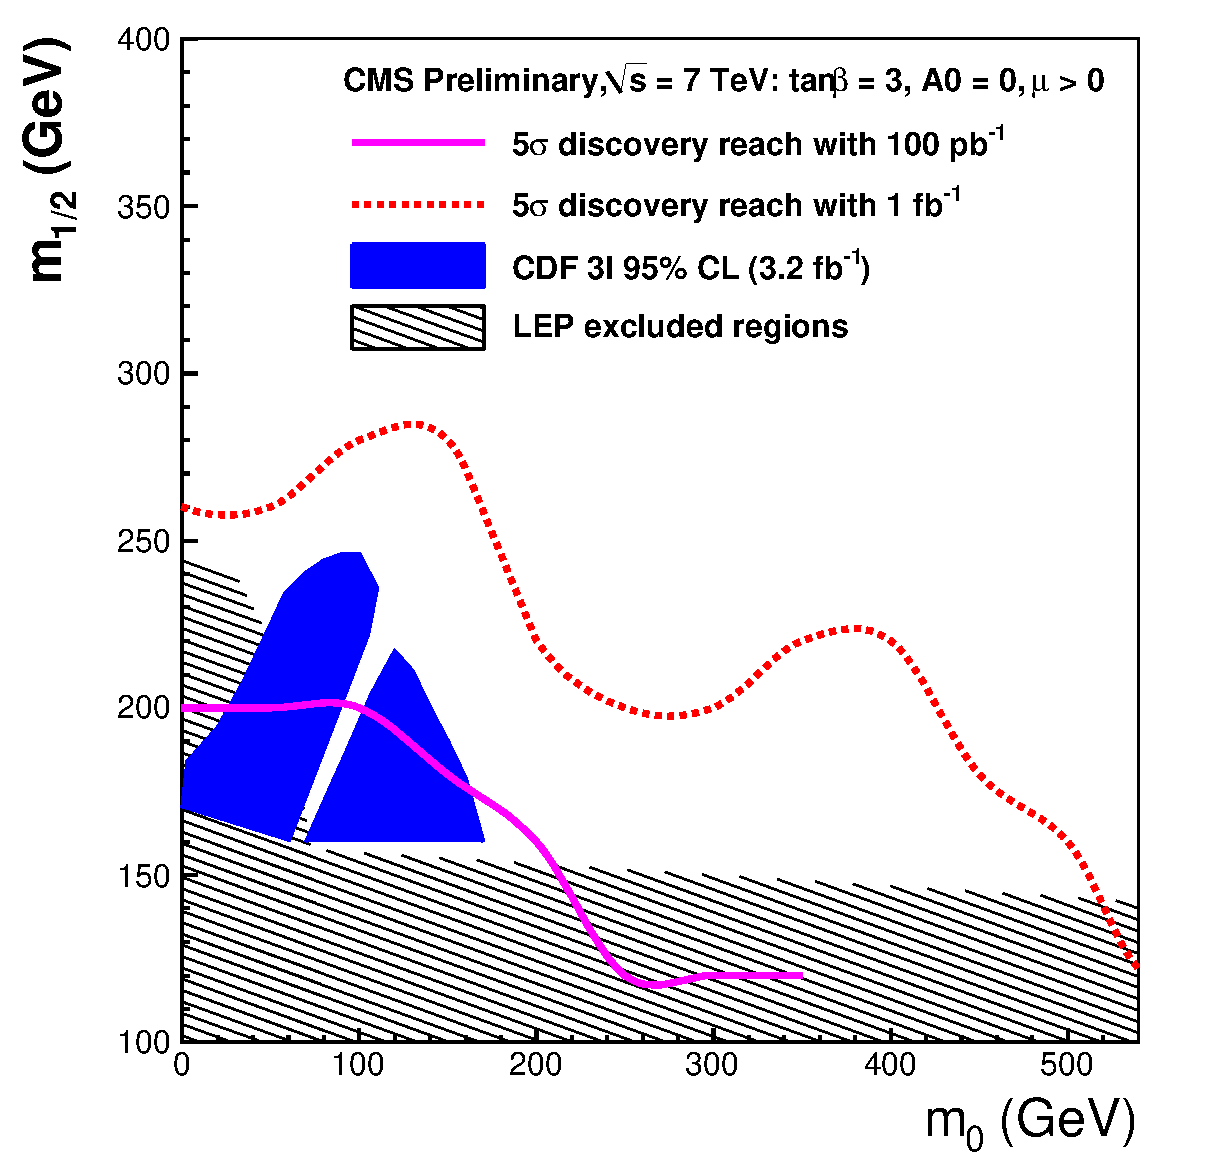
\includegraphics[width=0.7\linewidth]{figs/massreachss_zn.eps}
\caption{Discovery reach using significance estimated by $Z_N$~\cite{cite:conway} 
in the mSUGRA $m_{0}-m_{1/2}$ plane with tan$\beta = 3$, A$_0 = 0$, $\mu > 0$. 
Curves are shown for different luminosity scenarios. The blue region was excluded by 
the CDF experiment~\cite{cdf:recentSusy} and the black hashed region was excluded by the LEP 
experiments~\cite{lep:lepsusyreach}.\label{fig:ss_zn}}
\end{center}
\end{figure}
\vspace{3 mm}
\begin{figure}[htb]
\begin{center}
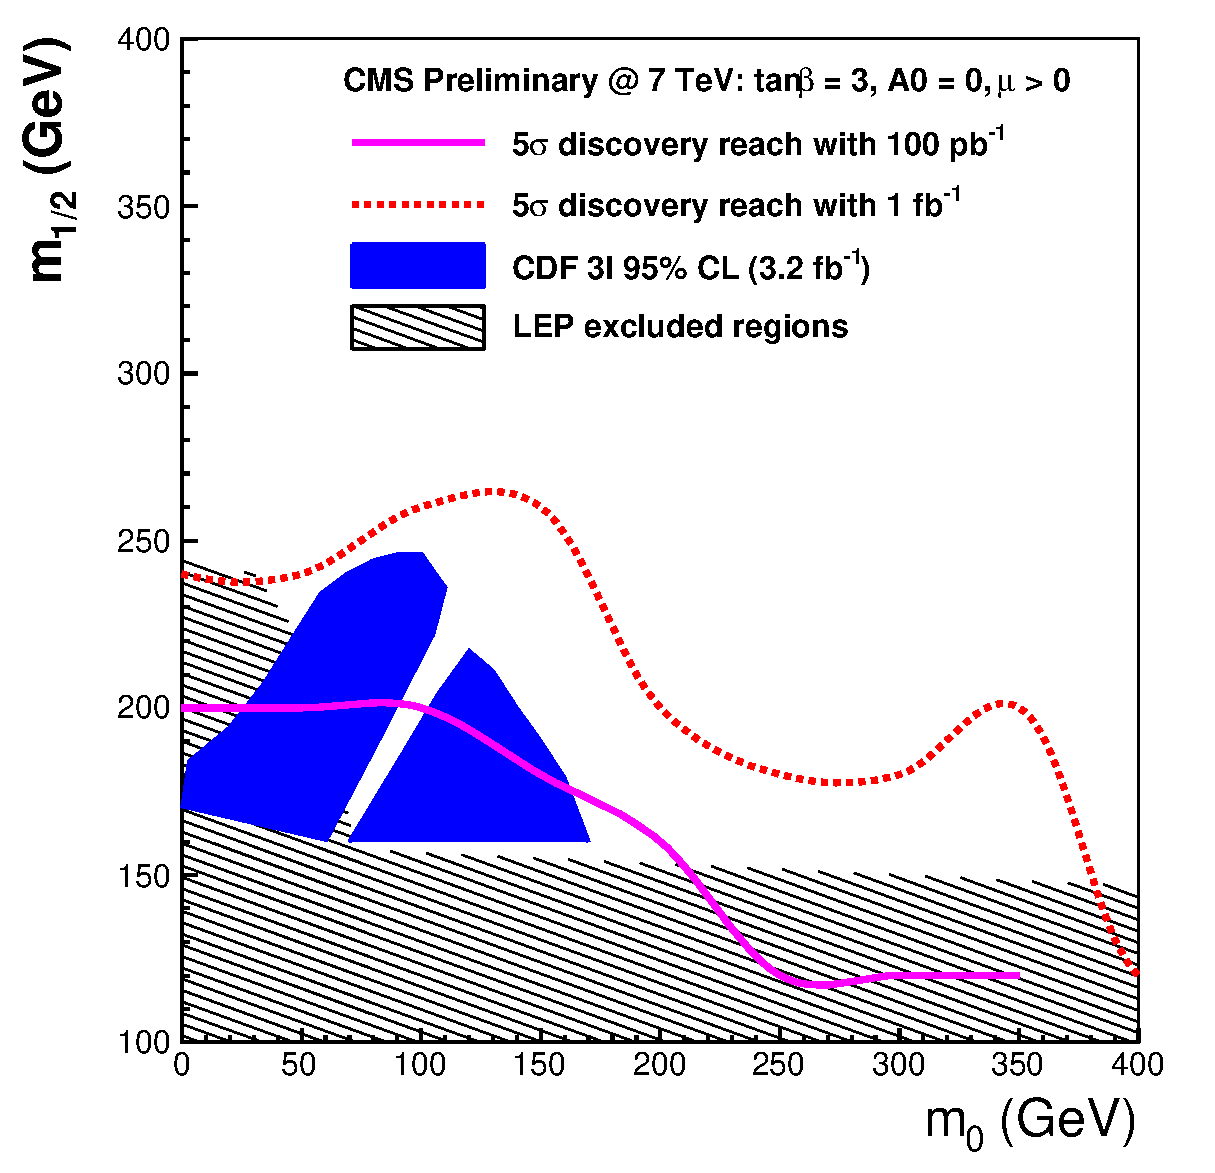
\includegraphics[width=0.7\linewidth]{figs/massreachss_bi.eps}
\caption{Discovery reach using significance estimated by $Z_{Bi}$~\cite{cite:cousins} 
in the mSUGRA $m_{0}-m_{1/2}$ plane with tan$\beta = 3$, A$_0 = 0$, $\mu > 0$. 
Curves are shown for different luminosity scenarios. The blue region was excluded by 
the CDF experiment~\cite{cdf:recentSusy} and the black hashed region was excluded by the LEP 
experiments~\cite{lep:lepsusyreach}.\label{fig:ss_zbi}}
\end{center}
\end{figure}



\subsection{Procedure for Excluding a Region of the mSUGRA Parameter Space}
\label{sec:exclusion}

Next we  determine the region of  the mSUGRA parameter  space which we
expect  to exclude  at 95\%  confidence level  (CL) if  we see
the SM expected yields in data. 
We  assume  that  we find  the  same
predicted background and observed yields in data  that we expect
to  find based on  our SM  MC. However, as the latter is 0.4, we computed  
for both an observation of 0 or 1 event in 100 pb$^{-1}$. We  use this  
information to  exclude a subset of the mSUGRA points using the following procedure.

The first  step is to  determine the 95\%  CL upper limit (UL)  on the
signal yield using a Bayesian method~\cite{bayes}. The required  inputs 
are: 

\begin{itemize}
\item The observed yield.
\item The relative  uncertainty in  the  signal acceptance (set  to 15\%).
\item The predicted  background yield.
\item Total  error  on the  predicted background yield (set to 50\%, unless otherwise stated).
\end{itemize}
We assume $0.4 \pm 0.6$ for background yield and its uncertainty.
\vspace{3 mm}
\begin{figure}[htb]
\begin{center}

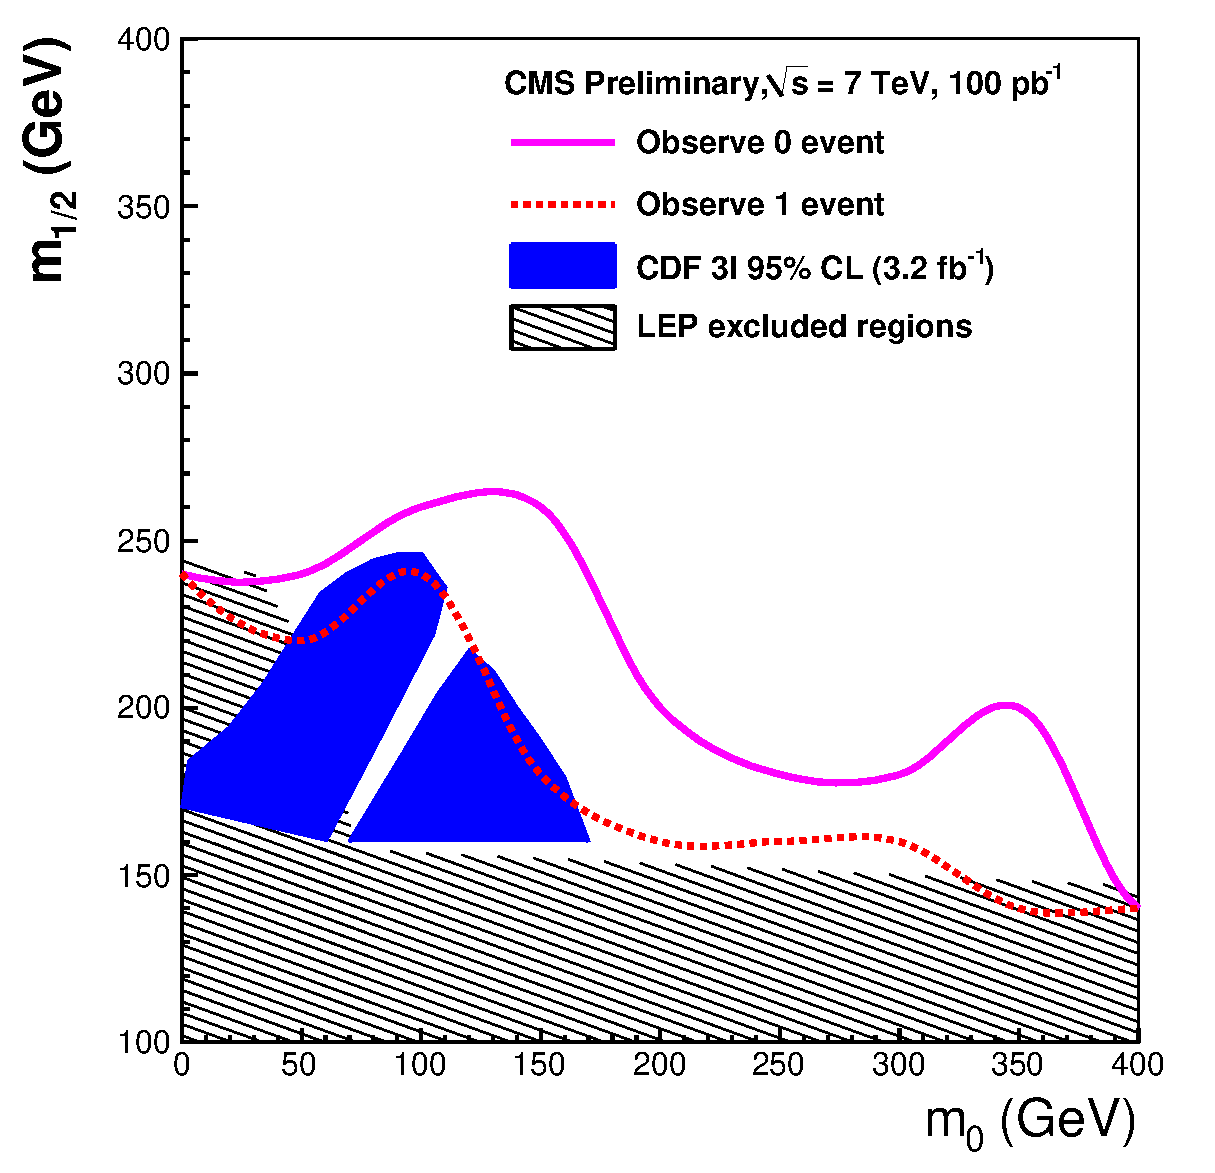
\includegraphics[width=0.485\linewidth]{figs/exclusion100ss.eps}
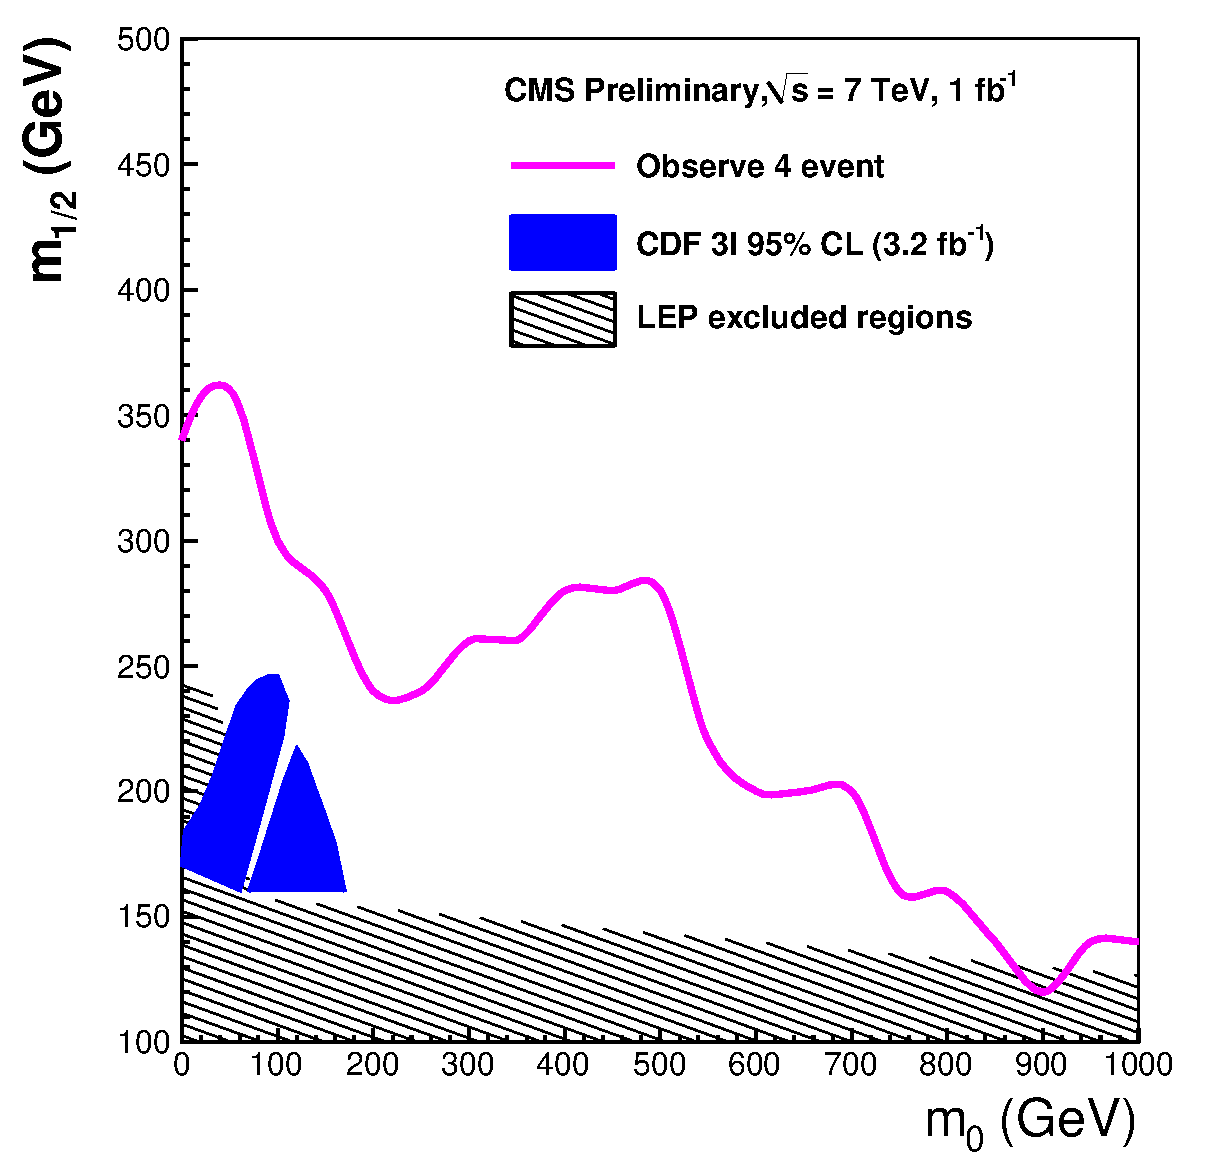
\includegraphics[width=0.485\linewidth]{figs/exclusion1fbss.eps}
\caption{The $m_{0}-m_{1/2}$ exclusion plot at the 95\% CL in the framework of 
mSUGRA assuming R-parity conservation using an  integrated  luminosity of  
$100~\mathrm{pb}^{-1}$ (left) and $1~\mathrm{fb}^{-1}$ (right). The blue region
was excluded by the CDF experiment~\cite{cdf:recentSusy}. The black hashed region was excluded
by the LEP experiments~\cite{lep:lepsusyreach}.\label{fig:ss_exclusion}}

\end{center}
\end{figure}

These values lead to  95\% CL  ULs  of 3.2 and 4.7  signal  events respectively for an assumed 
observation of 0 or 1 events. For the $1~\mathrm{fb}^{-1}$ limit we follow the same procedure
and find $4.0 \pm 2.0$ to lead to a 95\% CL UL yield of 7.3.

Next, we  exclude mSUGRA  points based on the  signal yield UL as derived above. The most 
obvious  way to do  so is to  exclude points which  lead  to a  difference  between  
observed  yield and  predicted background yield  which exceeds the  UL on the signal  yield. 
Figure~\ref{fig:ss_exclusion} shows the exclusion regions at 
95\% CL in the $m_{0}-m_{1/2}$ plane using integrated luminosities of 100 pb$^{-1}$
and 1 fb$^{-1}$. At 100 pb$^{-1}$ of the integrated luminosity the excluded 
regions are comparable with the current Tevatron limits. However, with 1 fb$^{-1}$
of data this study superceeds the current limits by a factor of $\sim$ 2 in gluino 
mass and quite significantly in higher $m_{0}$ accessable regions. The estimated and raw 
event yields along with statistical errors from MC are given in 
Tables~\ref{tab:ssyields_ex0}-\ref{tab:ssyields_ex1fb}.



